
\begin{lrbox}{\headingbox}
\begin{tikzpicture}[thin, dashed, every node/.style={inner sep=0mm,
  outer sep=4.5pt, font=\footnotesize}]
\draw foreach \y in {1,2,...,7} {
  [xshift=-\y cm/2, yshift=-\y cm/3]
  (0,0) node (O-0) {\textast}
  foreach \x [remember=\x as \lastx (initially 0)] in {1,...,\y} {
    (\x,0) node (O-\x) {\textast}
    (O-\lastx) -- (O-\x)
  }
};
\path (-1/4,0)node(A){\textast}
       (1/4,0)node(B){\textast}
      (-1/6,1/3)node{\textast}
       (1/6,1/3)node{\textast}
      (-1/6,7/3)node{\textast}
       (1/6,7/3)node{\textast};
\draw (A) -- (B);
\path foreach \x in {2,3,...,6,8} { (0,\x/3)node{\textast} };
\end{tikzpicture}
\end{lrbox}

\newsavebox\EndBox
\sbox\EndBox{\rotatebox{180}{\usebox\headingbox}}

\begin{dialog}{螃蟹卡农}

\begin{figure}
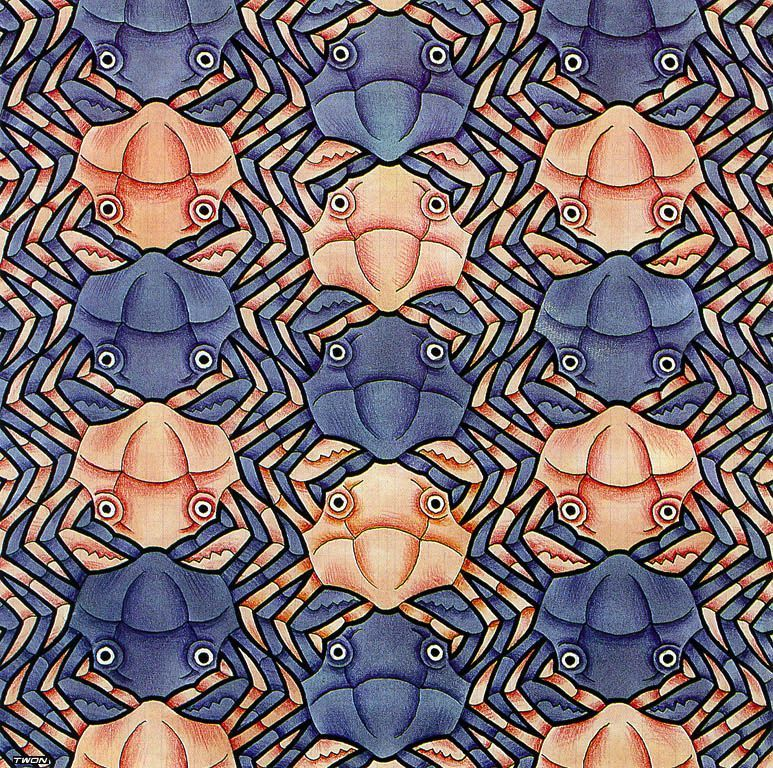
\includegraphics{img_042.jpg}
\caption{“螃蟹卡农”,艾舍尔作。}
\end{figure}

\begin{quote}
周末在公园散步时,乌龟碰巧遇见了阿基里斯。
\end{quote}

\begin{dialogue}

\item[乌龟]周末愉快,阿基。

\item[阿基里斯]彼此彼此。

\item[乌龟]同你在一起总是令人高兴的。

\item[阿基里斯]我也有同感。

\item[乌龟]在这样的天气里散步真是好极了,我宁愿散步回家。

\item[阿基里斯]哦,是吗?我觉得对你来说再没有比散步更好的了。

\item[乌龟]哎,阿基,这些天你看上去气色很好。

\item[阿基里斯]非常感谢。

\item[乌龟]不,不。来,尝尝我的荷兰雪茄吧。

\item[阿基里斯]啊,你在这方面真是个外行,你的口味不行。你不认为荷兰人的玩艺儿都很糟吗?

\item[乌龟]这点我可不同意。不过,说到口味,我终于看到了那位特别对你口味的艺术家艾舍尔的《螃蟹卡农》。那是有一天我在一家美术馆里看到的。我十分欣赏那种美和那种机巧:他把同一主题正向反向地罗织在一起。不过,我恐怕还是觉得巴赫要胜过艾舍尔。

\item[阿基里斯]这我不知道。但有一点可以肯定:我觉得讨论口味没劲。有句拉丁格言,恐怕你也知道:“口味无须争辩”。

\item[乌龟]告诉我,你这么大岁数了,觉得没劲了吗?

\item[阿基里斯]确切地说,是没多大力气了。

\item[乌龟]嗯,我也有这种感觉。

\item[阿基里斯]要是腿没力气了,就得拄手杖了。

\item[乌龟]你走路不使手杖吗?

\item[阿基里斯]我的一个朋友,他一向使。呆瓜。不过,我可从不沾惹手杖一根毛。

\dnote{(突然,螃蟹不知从哪儿冒了出来,用爪子指着一只青肿凸起的眼睛,神情激动地踅来踅去。)}

\item[螃蟹]好啊!好啊!怎么回事?怎么啦?你们瞧瞧这块青、这块肿,是一莽汉把我伤。嘿,而且是在这样一个好天里。你们瞧,我正在公园里懒洋洋地闲逛,迎面看到一个从彼得堡来的大块头——简直就是头熊——拿着一只吓人的俄国手杖。他足有三米高,除非我见了鬼。他那只手杖在地上划来划去,要不是我眼疾腿快,准被它打着了。于是我朝他爬过去,伸出爪子,打算拍拍他的膝盖,说,“对不起,先生,您用您的手杖把我们的公园老毛子化了。”可是,唔!他毫无幽默感——哪怕一丁、哪怕一星——噗!——他还放肆地敲了我一家伙,打在我眼睛上!按照我的本性,我原是横行无忌的,只是由于我们蟹类历来的传统,我原路退回了。毕竟,我们向前走时,就是倒着走。这是由于我们的基因,你们知道,它们是绕在一起的。这总是使我感到奇怪:究竟哪个在先——螃蟹还是基因?这也就是说,“哪个在后——基因还是螃蟹?”我总是绕圈子,你们知道。毕竟,这是由于我们的基因。我们倒着走时,就是向前走。呜呼!噫嘻!我得快快活活地颠儿了——在这样一个好天里。嘿,为螃蟹的生活叫好吧!再会!啊好!\dlnote{(他像出现时一样突然地消失了。)}

\begin{figure}[tb]
\fcapside[.35\columnwidth]{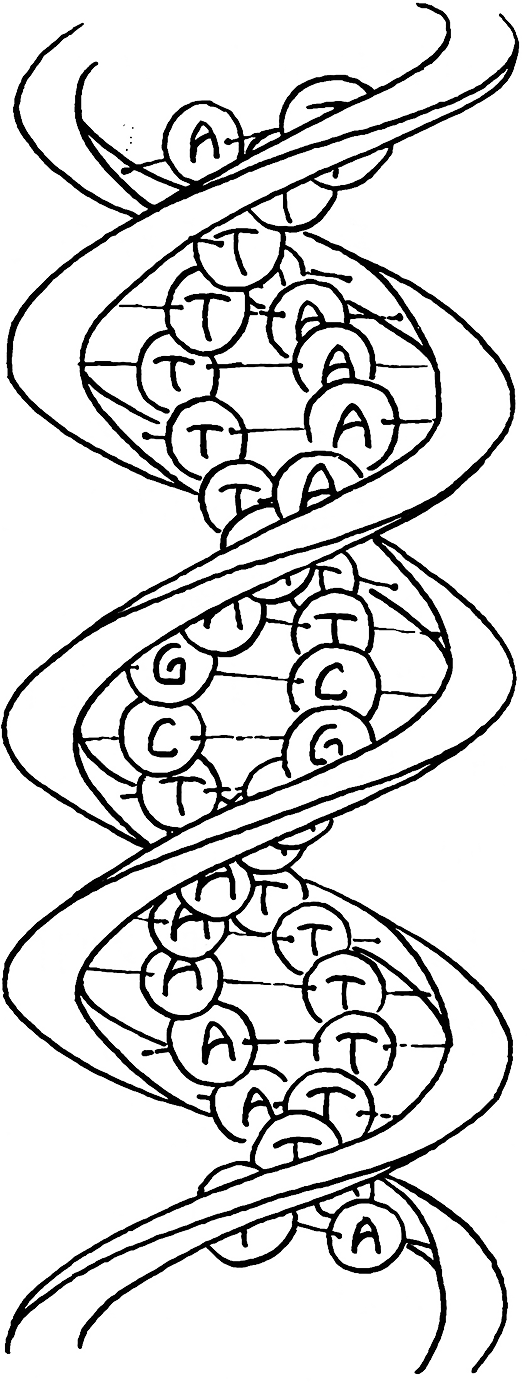
\includegraphics{img_043.png}}
{\caption[一小段螃蟹基因。]
{这里是螃蟹的一种基因中的一小段,它们一圈圈地缠绕着。当两股DNA链被拆开并且并排铺开时,它们读起来是这样的:\par
\centerline{\ldots TTTTTTTTTCGAAAAAAAAA\ldots}
\centerline{AAAAAAAAAGCTTTTTTTTT\ldots}
请注意它们是一模一样的,只是两者的走向正相反,一个前行时,另一个正好倒行。这正是音乐中所谓的“螃蟹卡农”这种形式所具有的特征。虽然不尽相同,它还是令人联想起回文来。回文就是一种正着读和倒着读都一模一样的句子。在分子生物学中,这样的DNA片段被称为“回文”——这种称呼有点用词不当,因为称它为“螃蟹卡农”要来得更准确些。不仅这个DNA片段是这样——而且本篇对话结构编排的基本序列也是螃蟹卡农式的。注意,在英文中,“阿基里斯”[Achilles]的第一个字母是A,“乌龟”[Tortoise]是T,“螃蟹”[Crab]是C,G则是“基因”[Gene]的第一个字母。}}
\end{figure}

\item[乌龟]我的一个朋友。他一向是呆瓜。不过我可从不沾惹老毛子的手杖。

\item[阿基里斯]你走路不使手杖吗?

\item[乌龟]要是腿没力气了,就得拄手杖了。

\item[阿基里斯]嗯,我也有这种感觉。

\item[乌龟]确切地说,是没有多大力气了。

\item[阿基里斯]告诉我,你这么大岁数了,觉得没劲了吗?

\item[乌龟]这我不知道。但有一点可以肯定:我觉得讨论口味没劲。有句拉丁格言,恐怕你也知道:“口味无须争辩”。

\item[阿基里斯]这点我可不同意。不过,说到口味,我终于听到了那位特别对你口味的作曲家巴赫的《螃蟹卡农》。那是有一天我在一次音乐会上听到的。我十分欣赏那种美和那种机巧:他把同一主题正向反向地罗织在一起。不过,我恐怕还是觉得艾舍尔要胜过巴赫。

\begin{sidewaysfigure}
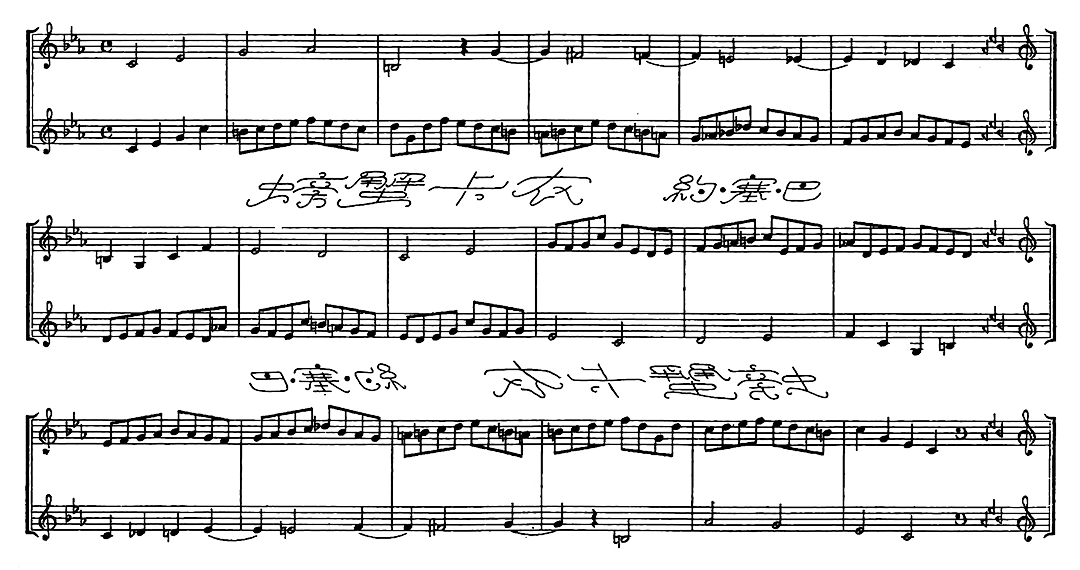
\includegraphics{img_044.png}
\caption[《螃蟹卡农》,选自巴赫《音乐的奉献》。]
  {《螃蟹卡农》,选自巴赫《音乐的奉献》。[乐谱是用唐纳德·伯德的程序“斯马特”印制的,美术字由陈春光设计。]}
\end{sidewaysfigure}

\item[乌龟]啊,你在这方面真是个外行,你的口味不行。你不认为荷兰人的玩艺儿都很糟吗?

\item[阿基里斯]不,不。来,尝尝我的荷兰雪茄吧。

\item[乌龟]非常感谢。

\item[阿基里斯]哎,龟兄,这些天你看去气色很好。

\item[乌龟]哦,是吗?我觉得对你来说再没有比散步更好的了。

\item[阿基里斯]在这样的天气里散步真是好极了,我宁愿散步回家。

\item[乌龟]我也有同感。

\item[阿基里斯]同你在一起总是令人高兴的。

\item[乌龟]彼此彼此。

\item[阿基里斯]周末愉快,龟兄。

\end{dialogue}

\begin{center}
\noindent\box\EndBox
\end{center}

\end{dialog}
